\section{Pulse Truncation and Endpoint Amplitude}
\label{sec:pulse-cutoff}

The ideal Lorentzian tail has infinite support, whereas the implemented pulse
starts and ends at finite amplitude $\Omega_c=c\Omega_0$.  Abruptly switching
this residual drive produces an endpoint transient.  A useful estimate of the
associated population contribution is~\cite{mihov_defying_2024}
\begin{equation}
    P_c(\Delta)
    \simeq
    \frac{\Omega_c^2}{\Omega_c^2+\Delta^2}
    \left[1-P_0(\Delta)\right],
    \qquad \Omega_c=c\Omega_0,
    \label{eq:cutoff-artifact}
\end{equation}
where $P_0$ denotes the response that would be obtained without the endpoint
jump.  The artifact becomes important when $\Omega_c$ is comparable to the
linewidth scale of interest.  Thus the cutoff cannot be assessed from $c$
alone: it must be considered together with the peak drive and the desired
resolution.

The Bloch-equation reference gives the dimensionless endpoint saturation
parameter
\begin{equation}
    s_c=\Omega_c^2T_1T_2.
    \label{eq:cutoff-saturation}
\end{equation}
Keeping the endpoint contribution in the weak-saturation regime requires
\begin{equation}
    s_c\ll1
    \quad\Longleftrightarrow\quad
    \Omega_c\ll\frac{1}{\sqrt{T_1T_2}}
    \quad\Longleftrightarrow\quad
    c\ll\frac{1}{\Omega_0\sqrt{T_1T_2}}.
    \label{eq:cutoff-inequality}
\end{equation}
The inequality therefore bounds the endpoint amplitude from above.  It is a
perturbative design criterion, not a claim that the cutoff artifact has the
steady-state Lorentzian lineshape.

We therefore measured the cutoff dependence over two complementary q1
echo--root--Lorentzian scans.  The broad survey spans $c=0.002$--$0.99$
with 25 peak-amplitude settings, while the focused sweep resolves
$c=0.01$--$0.10$ with 200 peak-amplitude settings.  Both use a
$20~\mu\mathrm{s}$ pulse and the same measured transverse-coherence
reference, $T_2=6.856~\mu\mathrm{s}$.
Fig.~\ref{fig:echo-lorentzian-cutoff-sweep}
reports the dimensionless reciprocal-linewidth metric
\begin{equation}
    \mathcal{R}
    = \frac{\Gamma_{f,T_2}}{\Gamma_f}
    = \frac{1/(\pi T_2)}{\Gamma_f},
    \label{eq:cutoff-resolution-metric}
\end{equation}
where every linewidth is a cyclic-frequency FWHM in hertz.  Thus
$\mathcal{R}=1$ is the $T_2$-limited linewidth and
$\mathcal{R}<1$ denotes a broader feature.  We also show the
signal-weighted metric $|A_{\mathrm{fit}}|\mathcal{R}$, which suppresses
narrow fits with negligible contrast.  These are linewidth-based scores, not
direct estimates of frequency-estimation uncertainty.

The maps retain only resolved and bounded probability features: the fitted
contrast is between 0.05 and 1, $R^2\geq0.60$, the fitted center lies inside
the measured frequency interval, and the FWHM lies between two frequency bins
and half the sweep span.  Gray cells denote measurements for which the fit did
not pass this common screen.  The denser focused sweep provides substantially
more accepted fits than the coarse survey and resolves the loss of reciprocal
linewidth performance as the cutoff increases across the $0.01$--$0.10$
interval.

\begin{figure}[t]
    \centering
    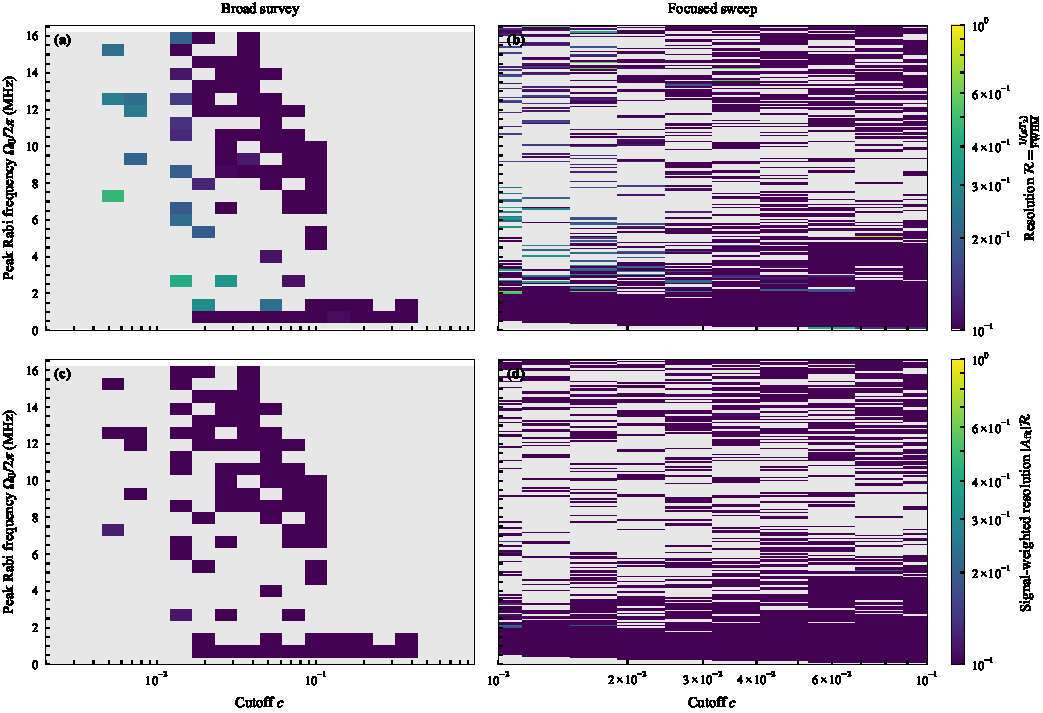
\includegraphics[width=\linewidth]{../figures/paper/08_echo_lorentzian_cutoff_sweep.pdf}
    \caption{Experimental cutoff sweep for q1 echo--root--Lorentzian
    spectroscopy.  The left column is the broad survey
    ($c=0.002$--$0.99$, 25 amplitudes, 60 repetitions per point); the right
    column is the denser focused sweep ($c=0.01$--$0.10$, 200 amplitudes,
    100 repetitions per point).
    (a,b) Reciprocal-linewidth metric $\mathcal{R}$ and
    (c,d) signal-weighted metric $|A_{\mathrm{fit}}|\mathcal{R}$.
    Both color scales are logarithmic.  On the upper color scale,
    $\mathcal{R}=1$ is the $T_2$-limited linewidth and values below one
    correspond to FWHM broader than that limit.  Gray cells are rejected or
    unresolved fits under the common screen described in the text; no fitted
    surface or interpolation is shown.}
    \label{fig:echo-lorentzian-cutoff-sweep}
\end{figure}
\FloatBarrier

\subsection{Simulated cutoff--amplitude operating map}

The finite-duration pulse is specified by its duration, peak drive amplitude,
and cutoff level.  To isolate the latter two parameters, we fix the pulse
duration at $50~\mu\mathrm{s}$ and simulate the root-Lorentzian and
echo-root-Lorentzian protocols over matched amplitude--cutoff grids.  For each
simulated spectrum, we extract the cyclic-frequency FWHM $\Gamma_f$ and the
contrast-weighted width
$\Gamma_f/(A_{\mathrm{peak}}\Gamma_{f,T_2})$.  This is a heuristic
resolution--signal metric; a direct Fisher-information or Cram\'er--Rao
analysis would additionally require a measurement-noise model and the full
frequency dependence of the response.

Fig.~\ref{fig:cutoff-parameter-map} shows that the root-Lorentzian pulse
contains extended narrow-linewidth regions, but its useful operating structure
is strongly oscillatory.  The echo protocol instead produces a broader,
contiguous region in which both the linewidth and the resolution--signal
trade-off remain favorable.  The logarithmic parameter axes should be kept in
mind when comparing the apparent area of these regions.

\begin{figure}[!ht]
    \centering
    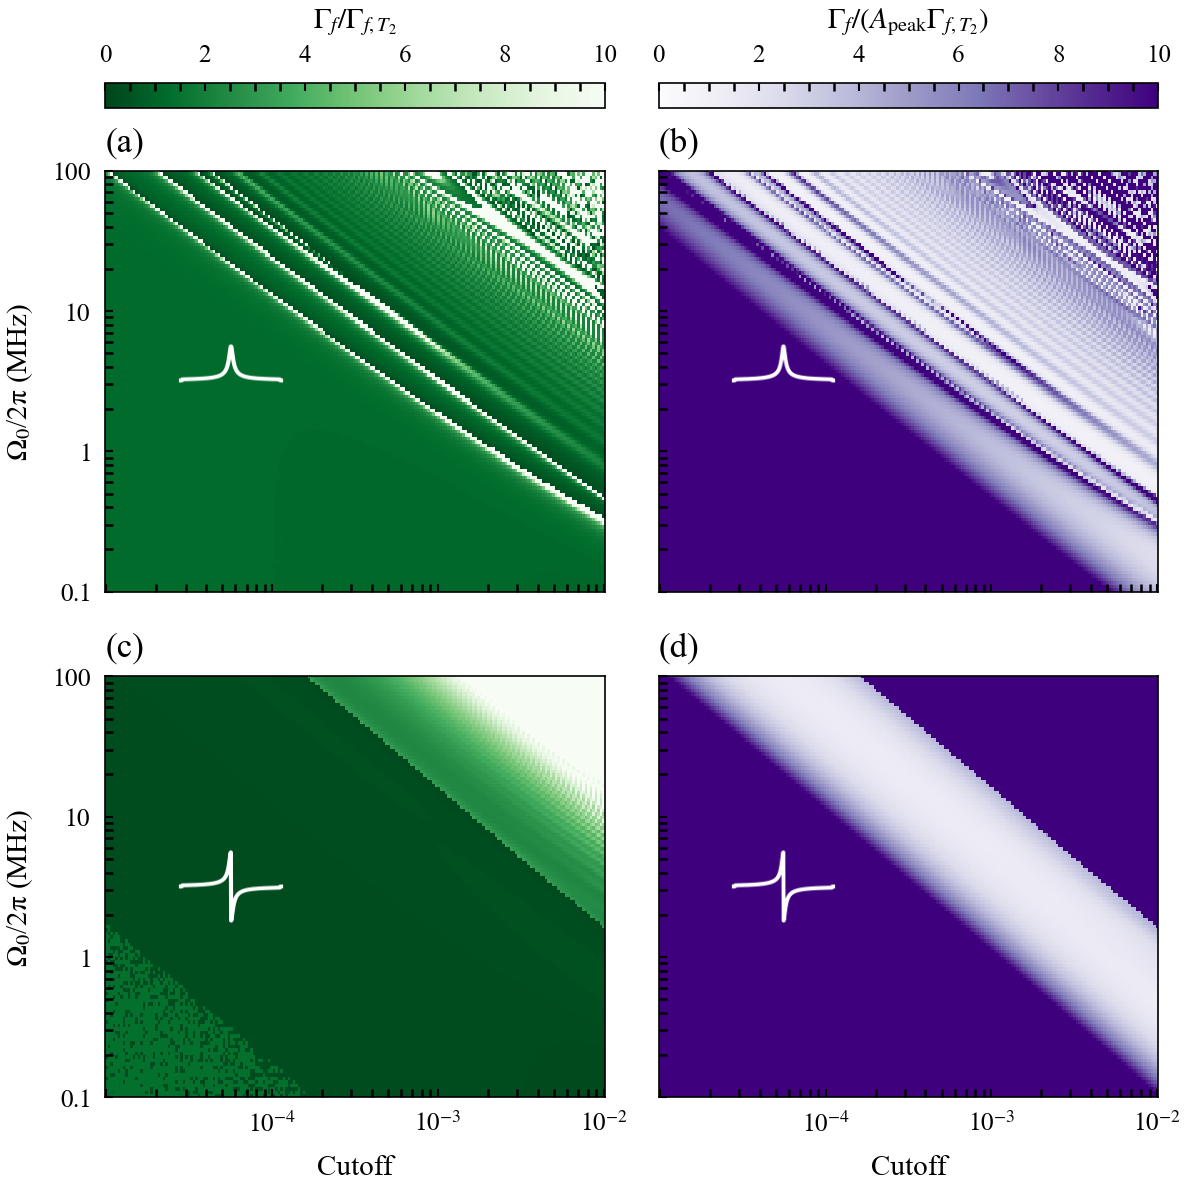
\includegraphics[width=0.72\textwidth]{../figures/paper/spectroscopy_fwhm_snr_vs_amplitude_vs_cutoff_2x2.png}
    \caption{Numerical cutoff--amplitude maps for root-Lorentzian $L^{(1/2)}$
    and echo-root-Lorentzian $L^{(1/2)}_{\mathrm{echo}}$ pulses of duration
    $50~\mu\mathrm{s}$.  (a,c) Normalized cyclic-frequency FWHM
    $\Gamma_f/\Gamma_{f,T_2}$ for the root and echo protocols, respectively;
    (b,d) corresponding contrast-weighted widths
    $\Gamma_f/(A_{\mathrm{peak}}\Gamma_{f,T_2})$.  The ordinary root-Lorentzian
    response is strongly oscillatory, whereas the echo variant retains a
    broader contiguous region with a favorable resolution--signal trade-off.}
    \label{fig:cutoff-parameter-map}
\end{figure}
\FloatBarrier
